\begin{figure}[H]
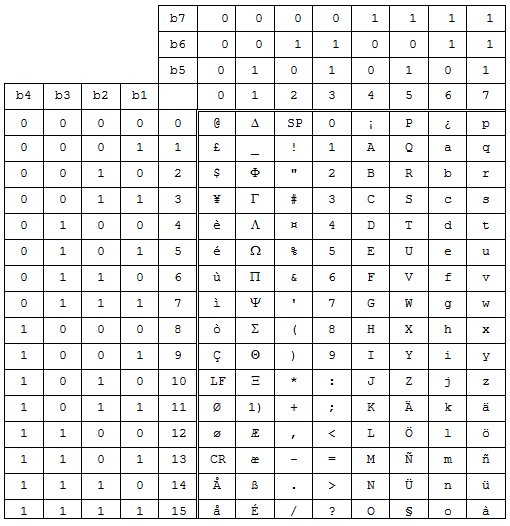
\includegraphics []{Billeder/tegnsaet.png}
\caption {Her ses skemaet for bit 7 tegnsættet. Ved 0x1b ses tegnet 1), der er et escape tegn til den ekstra tabel, som ses på figur \ref{tegnsaet2}}
\label {tegnsaet}
\end{figure}

\begin{figure}[H]
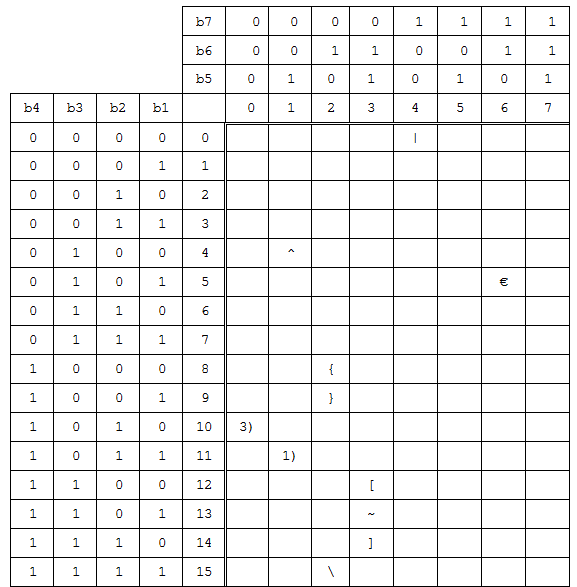
\includegraphics []{Billeder/tegnsaet2.png}
\caption {Den ekstra tabel for bit 7 tegnsaettet. Det samme tegn 1), er her et escape tegn som er reserveret hvis en ny ekstra tabel introduceres. Tegnet 3) er et form feed tegn, som er et escape tegn der starter en ny side.}
\label {tegnsaet2}
\end{figure}

\begin{figure}[H]
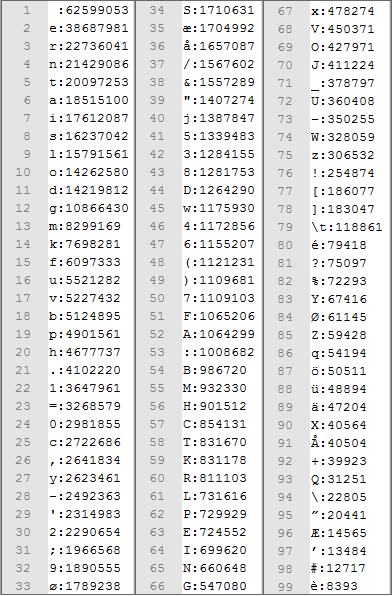
\includegraphics []{Billeder/wikiBilag.png}
\caption {Figuren viser et uddrag af vores wikipedia analyse af over 340.000 artikler.}
\label {wikiAnalyse}
\end{figure}

\begin{figure}[H]
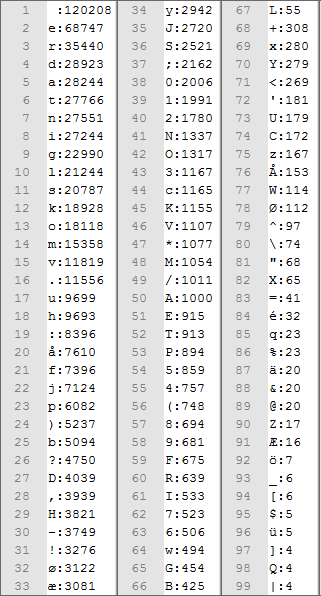
\includegraphics []{Billeder/SMSbilag.png}
\caption {Figuren viser hele vores SMS analyse af over 13.000 SMS beskeder}
\label {SMSanalyse}
\end{figure}

